% Options for packages loaded elsewhere
\PassOptionsToPackage{unicode}{hyperref}
\PassOptionsToPackage{hyphens}{url}
%
\documentclass[
]{article}
\usepackage{lmodern}
\usepackage{amssymb,amsmath}
\usepackage{ifxetex,ifluatex}
\ifnum 0\ifxetex 1\fi\ifluatex 1\fi=0 % if pdftex
  \usepackage[T1]{fontenc}
  \usepackage[utf8]{inputenc}
  \usepackage{textcomp} % provide euro and other symbols
\else % if luatex or xetex
  \usepackage{unicode-math}
  \defaultfontfeatures{Scale=MatchLowercase}
  \defaultfontfeatures[\rmfamily]{Ligatures=TeX,Scale=1}
\fi
% Use upquote if available, for straight quotes in verbatim environments
\IfFileExists{upquote.sty}{\usepackage{upquote}}{}
\IfFileExists{microtype.sty}{% use microtype if available
  \usepackage[]{microtype}
  \UseMicrotypeSet[protrusion]{basicmath} % disable protrusion for tt fonts
}{}
\makeatletter
\@ifundefined{KOMAClassName}{% if non-KOMA class
  \IfFileExists{parskip.sty}{%
    \usepackage{parskip}
  }{% else
    \setlength{\parindent}{0pt}
    \setlength{\parskip}{6pt plus 2pt minus 1pt}}
}{% if KOMA class
  \KOMAoptions{parskip=half}}
\makeatother
\usepackage{xcolor}
\IfFileExists{xurl.sty}{\usepackage{xurl}}{} % add URL line breaks if available
\IfFileExists{bookmark.sty}{\usepackage{bookmark}}{\usepackage{hyperref}}
\hypersetup{
  pdftitle={Sensor-guided Side-dressing Decision Making},
  pdfauthor={Taro Mieno and John Doe},
  hidelinks,
  pdfcreator={LaTeX via pandoc}}
\urlstyle{same} % disable monospaced font for URLs
\usepackage[margin=1in]{geometry}
\usepackage{graphicx}
\makeatletter
\def\maxwidth{\ifdim\Gin@nat@width>\linewidth\linewidth\else\Gin@nat@width\fi}
\def\maxheight{\ifdim\Gin@nat@height>\textheight\textheight\else\Gin@nat@height\fi}
\makeatother
% Scale images if necessary, so that they will not overflow the page
% margins by default, and it is still possible to overwrite the defaults
% using explicit options in \includegraphics[width, height, ...]{}
\setkeys{Gin}{width=\maxwidth,height=\maxheight,keepaspectratio}
% Set default figure placement to htbp
\makeatletter
\def\fps@figure{htbp}
\makeatother
\setlength{\emergencystretch}{3em} % prevent overfull lines
\providecommand{\tightlist}{%
  \setlength{\itemsep}{0pt}\setlength{\parskip}{0pt}}
\setcounter{secnumdepth}{-\maxdimen} % remove section numbering
\newlength{\cslhangindent}
\setlength{\cslhangindent}{1.5em}
\newenvironment{cslreferences}%
  {}%
  {\par}

\title{Sensor-guided Side-dressing Decision Making}
\author{Taro Mieno\footnote{University of Nebraska Lincoln,
  \href{mailto:tmieno2@unl.edu}{\nolinkurl{tmieno2@unl.edu}}} and John
Doe\footnote{Random University,
  \href{mailto:johndoe@email.com}{\nolinkurl{johndoe@email.com}}}}
\date{2020-11-11}

\begin{document}
\maketitle
\begin{abstract}
Abstract: this research is so awesome that you cannot reject this paper.
\end{abstract}

\hypertarget{introduction}{%
\section{Introduction}\label{introduction}}

The issue this article addresses is \textbf{super} \emph{important}!

{[}1{]} examined bluh bluh.

bluh bluh {[}2{]}

bluh bluh {[}1,2{]}

bluh bluh {[}2{]}

\hypertarget{page-break-you-cannot-see-this-text-on-the-output-word-file}{%
\subparagraph{page break (you cannot see this text on the output WORD
file)}\label{page-break-you-cannot-see-this-text-on-the-output-word-file}}

\hypertarget{materials-and-methods}{%
\section{Materials and Methods}\label{materials-and-methods}}

This line break does not work: See?

This line break does work:

See?

\hypertarget{data}{%
\subsection{Data}\label{data}}

The number of observations are 598 and 1376 for Zones 2 and 3,
respectively.

Table @ref(tab:table-1) presents summary statistics by zone.

\hypertarget{statistical-model}{%
\subsection{Statistical Model}\label{statistical-model}}

Here is the statistical model to estimate:

Equations written in the \texttt{aligned} environment.

\[
\begin{aligned}
 Y_z & = f_z(S) + g_z(N) + h_z(X,Y) + \varepsilon_z \\
& = \sum_{i=1}^k \phi_k(S) + g_z(N) + h_z(X,Y) + \varepsilon_z
\end{aligned}
\]

Equations written in the \texttt{align} environment.

\[
\begin{align}
 Y_z & = f_z(S) + g_z(N) + h_z(X,Y) + \varepsilon_z \\
& = \sum_{i=1}^k \phi_k(S) + g_z(N) + h_z(X,Y) + \varepsilon_z
\end{align}
\]

\hypertarget{results-and-discussions}{%
\section{Results and Discussions}\label{results-and-discussions}}

Table @ref(tab:table-1) presents the regression results.

Figure @ref(fig:fig-1) presents the distribution of yields by zone.

\hypertarget{conclusions}{%
\section{Conclusions}\label{conclusions}}

bluh blu\footnote{This is a footnote}

\hypertarget{figures}{%
\section{Figures}\label{figures}}

\begin{figure}

{\centering 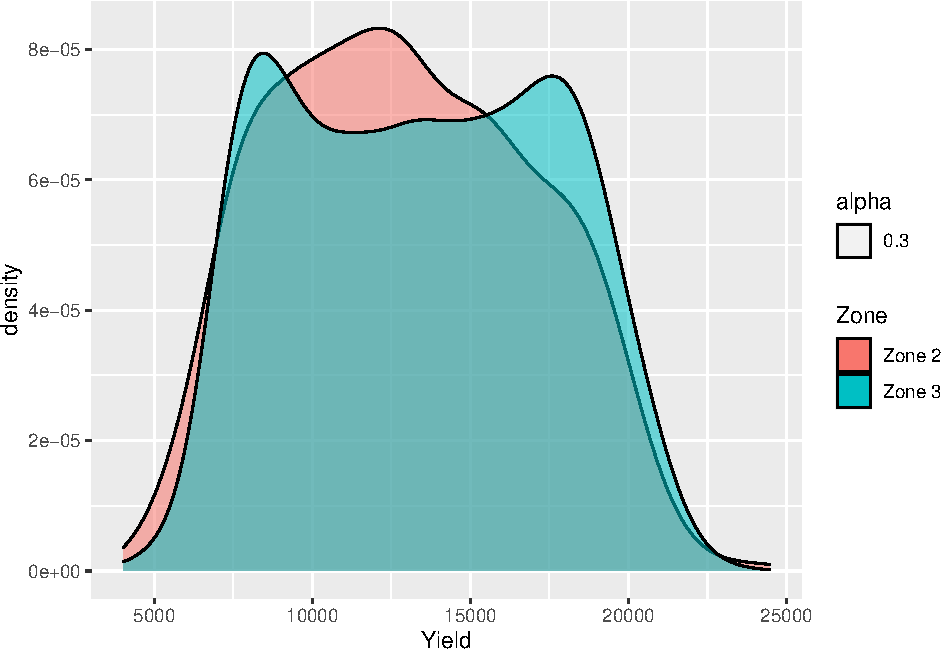
\includegraphics[width=468px]{sample_to_word_files/figure-latex/fig-1-1} 

}

\caption{The Distribution of Yield by Zone}\label{fig:fig-1}
\end{figure}

\hypertarget{tables}{%
\section{Tables}\label{tables}}

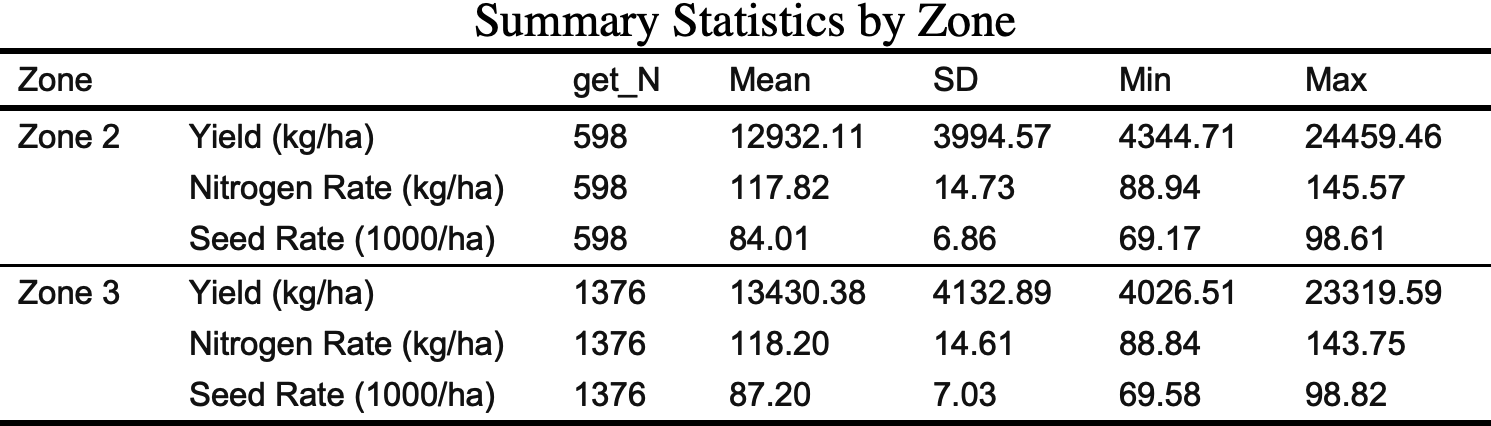
\includegraphics[width=6.72in,height=2.22in,keepaspectratio]{sample_to_word_files/figure-latex/table-1-1.png}

\hypertarget{references}{%
\section{References}\label{references}}

\hypertarget{refs}{}
\begin{cslreferences}
\leavevmode\hypertarget{ref-adrian2005producers}{}%
1. Adrian, A.M.; Norwood, S.H.; Mask, P.L. Producers' perceptions and
attitudes toward precision agriculture technologies. \emph{Computers and
electronics in agriculture} \textbf{2005}, \emph{48}, 256--271.

\leavevmode\hypertarget{ref-shrader1966estimation}{}%
2. Shrader, W.; Fuller, W.; Cady, F. Estimation of a common nitrogen
response function for corn (zea mays) in different crop rotations 1.
\emph{Agronomy Journal} \textbf{1966}, \emph{58}, 397--401.
\end{cslreferences}

\end{document}
